\documentclass{beamer}
\usepackage[spanish]{babel}
\usepackage{tikz}
\usepackage[utf8]{inputenc}
\mode<presentation>{}
\usepackage{beamerthemesplit} 
\setbeamertemplate{caption}[numbered]
%\setbeamertemplate{footline}[frame number]
\usetheme{Warsaw}
\usecolortheme{crane}
\useoutertheme{shadow}
\useinnertheme{rectangles}
\title[Online Game Servers]{Online Game Servers}
\subtitle{P2P game network analysis}
\author{Miguel Lentisco Ballesteros \\ José Antonio Álvarez Ocete}
\date{\today}


\AtBeginSection{ 
\begin{frame} 
  \frametitle{Index}
  \tableofcontents[currentsection]
\end{frame}
}

\AtBeginSubsection{ 
\begin{frame}
  \frametitle{Index}
  \tableofcontents[currentsection,currentsubsection]
\end{frame}
}

\beamertemplatenavigationsymbolsempty 

\expandafter\def\expandafter\insertshorttitle\expandafter{%
  \insertshorttitle\hfill%
  \insertframenumber\,/\,\inserttotalframenumber}

\begin{document}

\frame{\titlepage}

\begin{frame}
	\frametitle{Index}
	\tableofcontents
\end{frame}

\section{Online game servers}
\begin{frame}
	\frametitle{Game servers}
	\begin{block}{Questions}
		\begin{enumerate}
			\item How do they work?
			\item What transport protocols do they use?
			\item What types do they have?
		\end{enumerate}
	\end{block}
\end{frame}

\subsection{Server working}
\begin{frame}
	\frametitle{How do game servers work?}
	Simplified diagram: the client and the server.
	\begin{enumerate}
		\item The players moves from (1,0) to (3,0)
		\item The client sends this data to the server
		\item How the server deals with it?
	\end{enumerate}
\end{frame}

\begin{frame}
	\frametitle{Authoritative and non-authoritative}
	There are 2 approaches:
	\begin{itemize}
		\item \alert{Authoritative}: the server has the final say.
		\item \alert{Non-authoritative}: the client does not have to wait the server.
	\end{itemize}
	\pause
\end{frame}

\begin{frame}
	\frametitle{Problems}
	Two factors:
	\begin{itemize}
		\item \alert{Precision}
		\item \alert{Latency} \\~\\
	\end{itemize}
	Trade-off between both. \\~\\ 
 	\pause
	Client-side prediction.
\end{frame}

\begin{frame}
	\frametitle{Client-side prediction}
	\begin{figure}[H]
    	\centering
     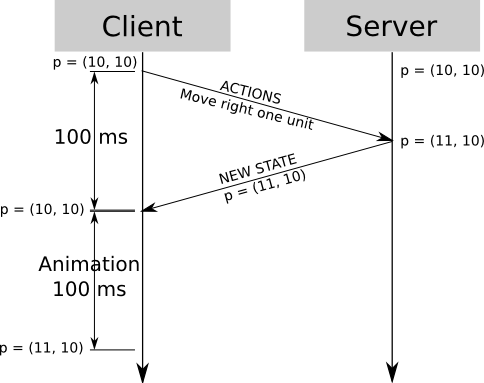
\includegraphics[width=0.6\textwidth]{prediction1.png}
     \caption{Without prediction}
     \end{figure}
\end{frame}

\begin{frame}
	\frametitle{Client-side prediction}
	\begin{figure}[H]
    	\centering
     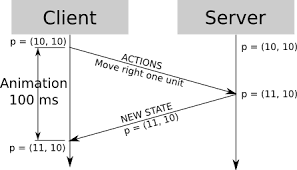
\includegraphics[width=0.8\textwidth]{prediction2.png}
     \caption{With prediction}
     \end{figure}
\end{frame}

\begin{frame}
	\frametitle{Client-side prediction}
	\begin{figure}[H]
    	\centering
     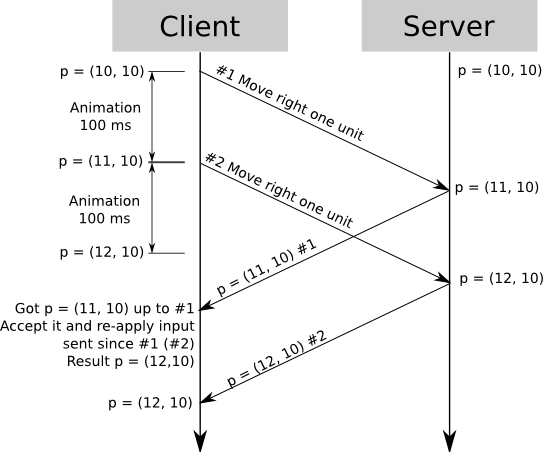
\includegraphics[width=0.65\textwidth]{prediction3.png}
     \caption{Prediction - server}
     \end{figure}
\end{frame}

\subsection{Transport protocols}
\begin{frame}
	\frametitle{UDP vs TCP}
	\begin{itemize}
		\item \alert{UDP}: FPS, MMO (ocassional lag not desirable)
		\item \alert{TCP}: RTS, Poker (ocassional delay doesn't affect)
	\end{itemize}
\end{frame}

\subsection{Game server types}
\begin{frame}
	\frametitle{Types}
	\begin{itemize}
		\item \alert{P2P}.
		\item \alert{Server-Client}: 
		\begin{itemize}
			\item Dedicated.
			\item Listen.
		\end{itemize}
	\end{itemize}
\end{frame}

\begin{frame}
	\frametitle{P2P}
	Each client recives the input of each other players. Used on RTS.
	\begin{figure}[H]
    	\centering
     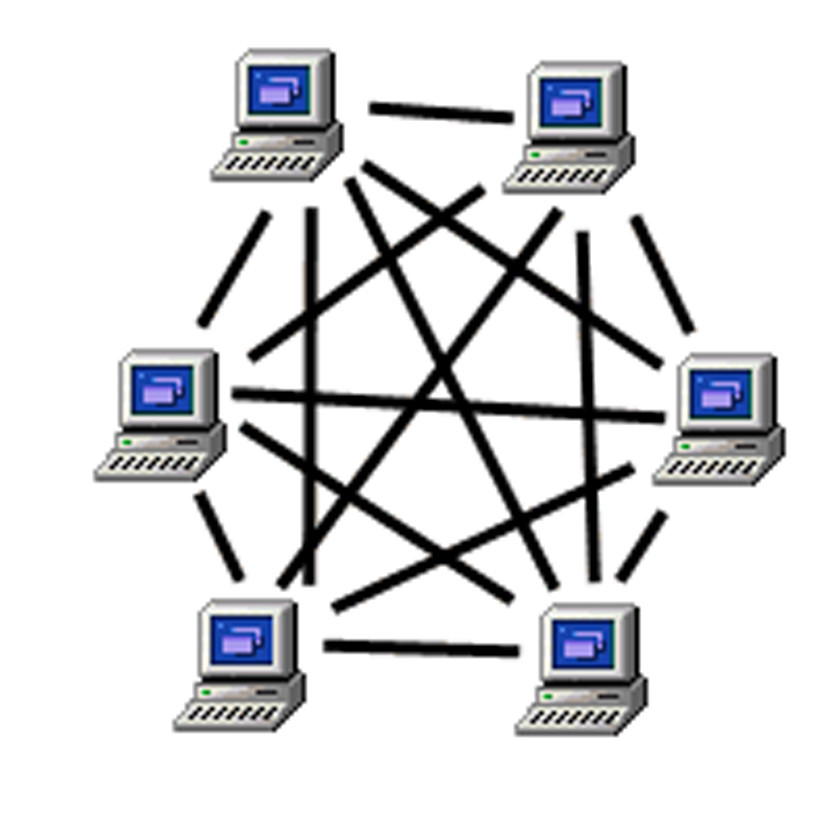
\includegraphics[width=0.5\textwidth]{p2p.jpg}
     \caption{P2P network}
     \end{figure}
\end{frame}

\begin{frame}
	\frametitle{Server-Client}
	\begin{figure}[H]
    	\centering
     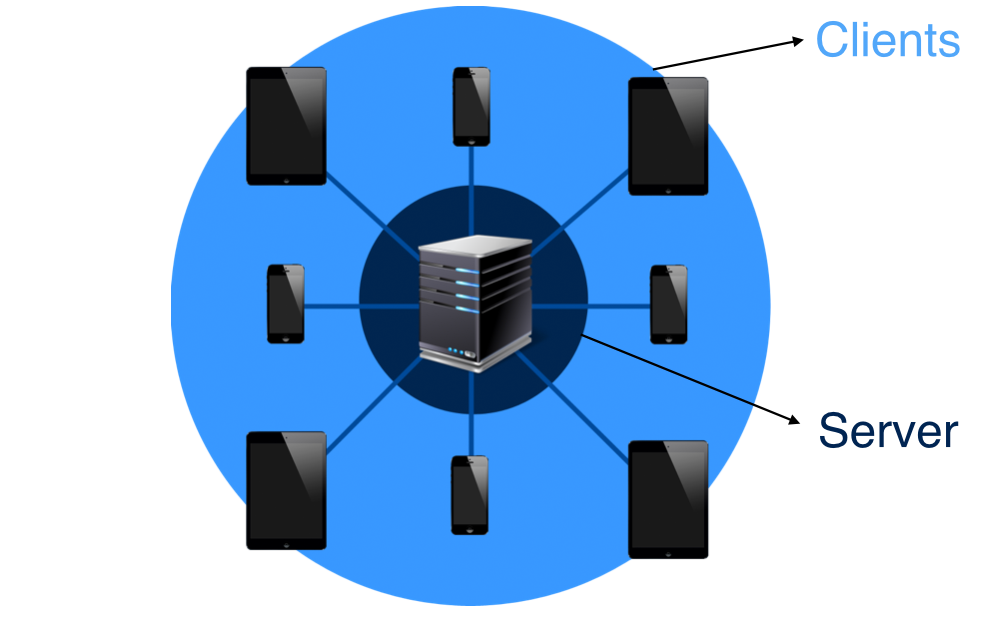
\includegraphics[width=0.8\textwidth]{clientserver.png}
     \caption{Client-server}
     \end{figure}
\end{frame}

\section{Our game server}
\subsection{Description}
\begin{frame}
	\frametitle{Description}
	\begin{block}{Server}
		Service implementing the Tic-Tac-Toe game online.
	\end{block}
	\begin{itemize}
		\item One concurrent server communicating with the clients via UDP.
		\item When there are at least 2 clients, the server matches them sending the address and port.
		\item The clients will play against each other via TCP.
	\end{itemize}
\end{frame}

\subsection{Diagram}
\begin{frame}
\frametitle{Connection diagram}
\begin{center}
\begin{tikzpicture}[scale=0.14]
\tikzstyle{every node}+=[inner sep=0pt]
\draw [black] (14.8,-26.4) circle (4);
\draw (14.8,-26.4) node {$Server$};
\draw [black] (37.3,-8.6) circle (4);
\draw (37.3,-8.6) node {$client1$};
\draw [black] (36.4,-45.7) circle (4);
\draw (36.4,-45.7) node {$client2$};
\draw [black] (15.785,-23.568) arc (157.29832:99.39751:24.409);
\fill [black] (15.79,-23.57) -- (16.56,-23.02) -- (15.63,-22.64);
\draw (14.35,-13.35) node [above] {$UDP\mbox{ }(want\mbox{ }play)$};
\draw [black] (35.73,-11.155) arc (-33.85383:-69.45035:37.714);
\fill [black] (35.73,-11.16) -- (34.87,-11.54) -- (35.7,-12.1);
\draw (38.01,-20.22) node [below] {$UDP\mbox{ }(client\mbox{ }2\mbox{ }data)$};
\draw [black] (33.404,-45.764) arc (-93.14281:-170.41995:19.685);
\fill [black] (15.07,-29.38) -- (14.71,-30.26) -- (15.7,-30.09);
\draw (12.55,-41.28) node [below] {$UDP\mbox{ }(want\mbox{ }play)$};
\draw [black] (17.508,-27.689) arc (62.69338:33.74387:46.427);
\fill [black] (34.82,-43.15) -- (34.79,-42.21) -- (33.96,-42.77);
\draw (37.36,-33.83) node [above] {$UDP\mbox{ }(client\mbox{ }2\mbox{ }data)$};
\draw [black] (40.291,-8.411) arc (89.05689:-91.8362:18.818);
\fill [black] (39.38,-46.03) -- (40.16,-46.56) -- (40.19,-45.56);
\draw (59.33,-27.69) node [right] {$TCP\mbox{ }(playing)$};
\draw [black] (40.291,-8.414) arc (88.98405:-91.76336:18.814);
\fill [black] (40.29,-8.41) -- (41.08,-8.93) -- (41.1,-7.93);
\end{tikzpicture}
\end{center}
\end{frame}

\subsection{Frame}
\begin{frame}
	\frametitle{Frame server}
	P2P network, non-authoritative server and TCP.
	\\~\\
	Precision over latency, datacheck in the client.
	\\~\\
	Server works as database.
\end{frame}


\section{Problems in real life}

\subsection{The question}
\begin{frame}
	\frametitle{Viability}
	\begin{block}{The question}
		Is viable to apply this structure to real games? 
	\end{block}
	\pause
	Yes, in fact it has been done already.
\end{frame}

\subsection{Old games}
\begin{frame}
	\frametitle{Problem}
	\begin{block}{Problem}
		Many old games are out of date but there are a lot of people playing them yet. How can they play online against each other?
	\end{block}
	Games:
	\begin{itemize}
		\item Age of Empires.
		\item Need for Speed.
		\item Civilization.
		\item Empire Earth.
		\item Worms.
		\item The Settlers.
		\item Call of Duty.
	\end{itemize}
\end{frame}

\subsection{Solution}

\begin{frame}
	\frametitle{The solution}
	\begin{block}{Solution}
		A server saving the data of people hosting games and giving the information to the other players who wants to connect.
	\end{block}
	\pause
	\begin{columns}
	\begin{column}{0.6\textwidth}
   GameRanger is a Internet gaming service that has resolved this problem since 1999, running with 726 games currently. Also, it offers other features as voicechat or chatrooms.
   
\end{column}
\begin{column}{0.4\textwidth}
    \begin{center}
    \begin{figure}[H]
     
\includegraphics[width=0.5\textwidth]{gameranger.png}
     \caption{GameRanger}
     \end{figure}
     \end{center}
\end{column}
\end{columns}
\end{frame}

\begin{frame}
	\frametitle{Example}
	\begin{figure}[H]
    	\centering
     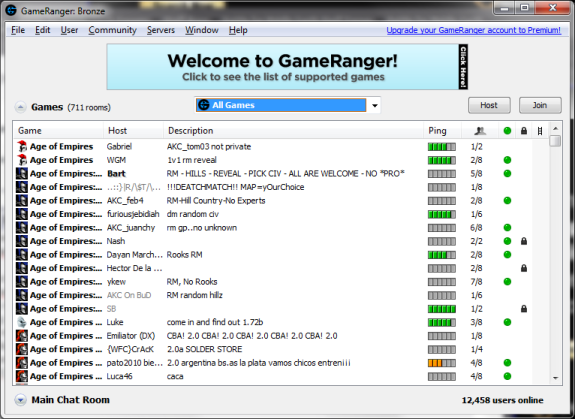
\includegraphics[width=0.75\textwidth]{gamerangerexample.png}
     \caption{GameRanger app}
     \end{figure}
\end{frame}

\section{Wireshark}
\begin{frame}
	\frametitle{Wireshark captures}
	\begin{figure}[H]
    	\centering
     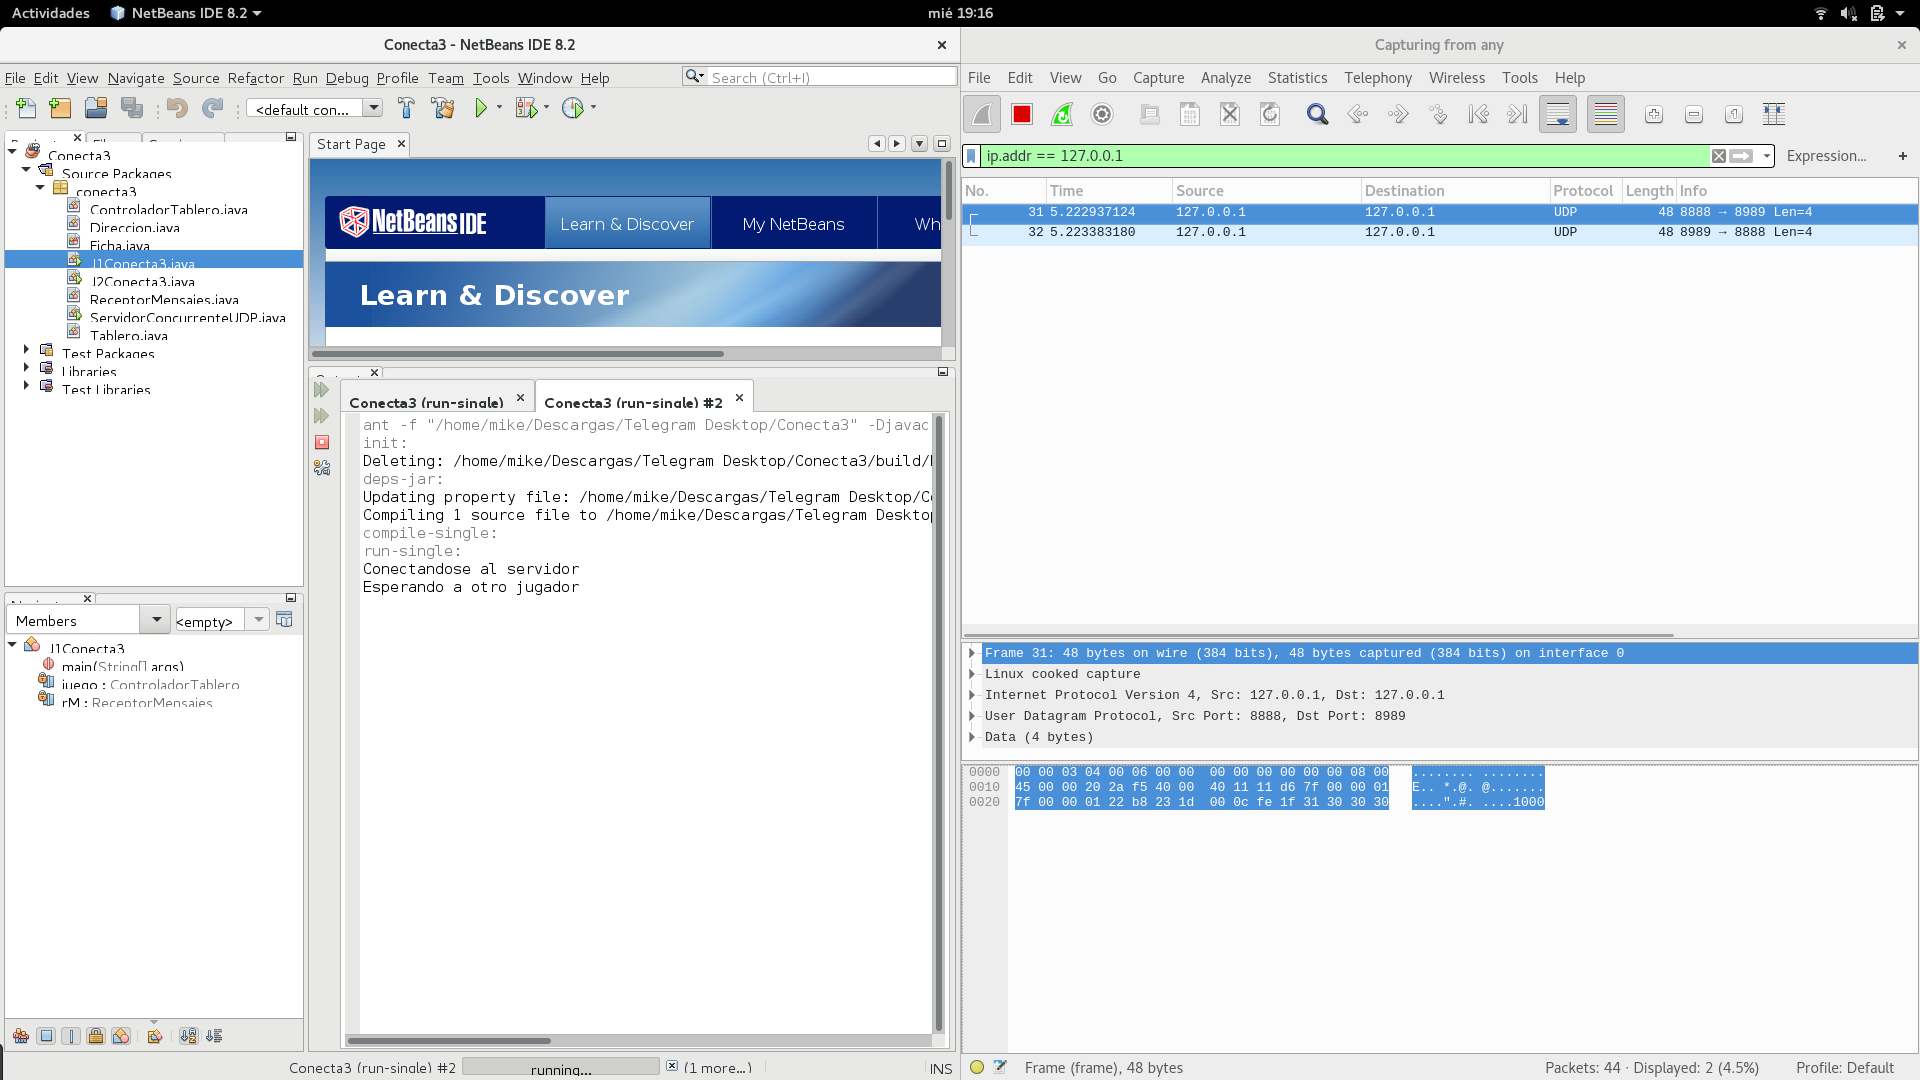
\includegraphics[width=0.9\textwidth]{1.png}
     \caption{Client hello}
     \end{figure}
\end{frame}

\begin{frame}
	\frametitle{Wireshark captures}
	\begin{figure}[H]
    	\centering
     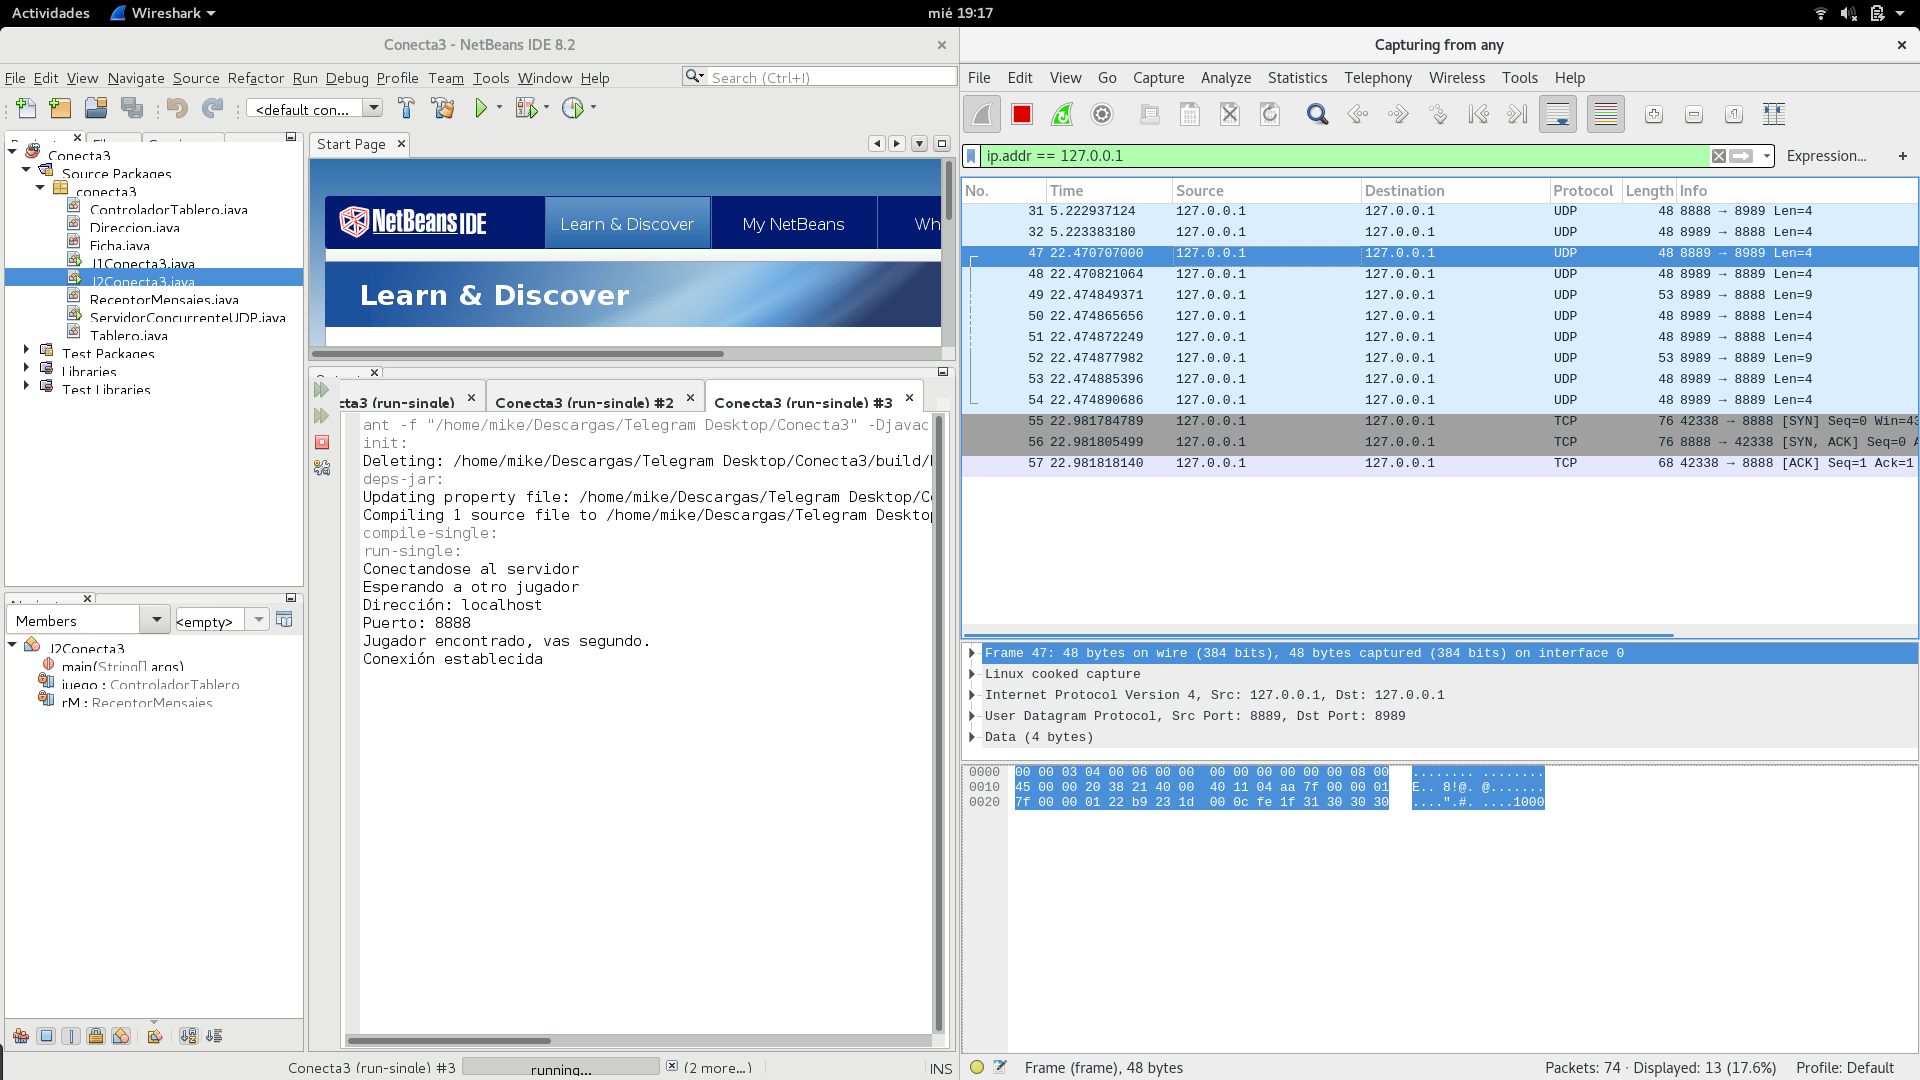
\includegraphics[width=0.9\textwidth]{2.png}
     \caption{Conexion accepted}
     \end{figure}
\end{frame}

\begin{frame}
	\frametitle{Wireshark captures}
	\begin{figure}[H]
    	\centering
     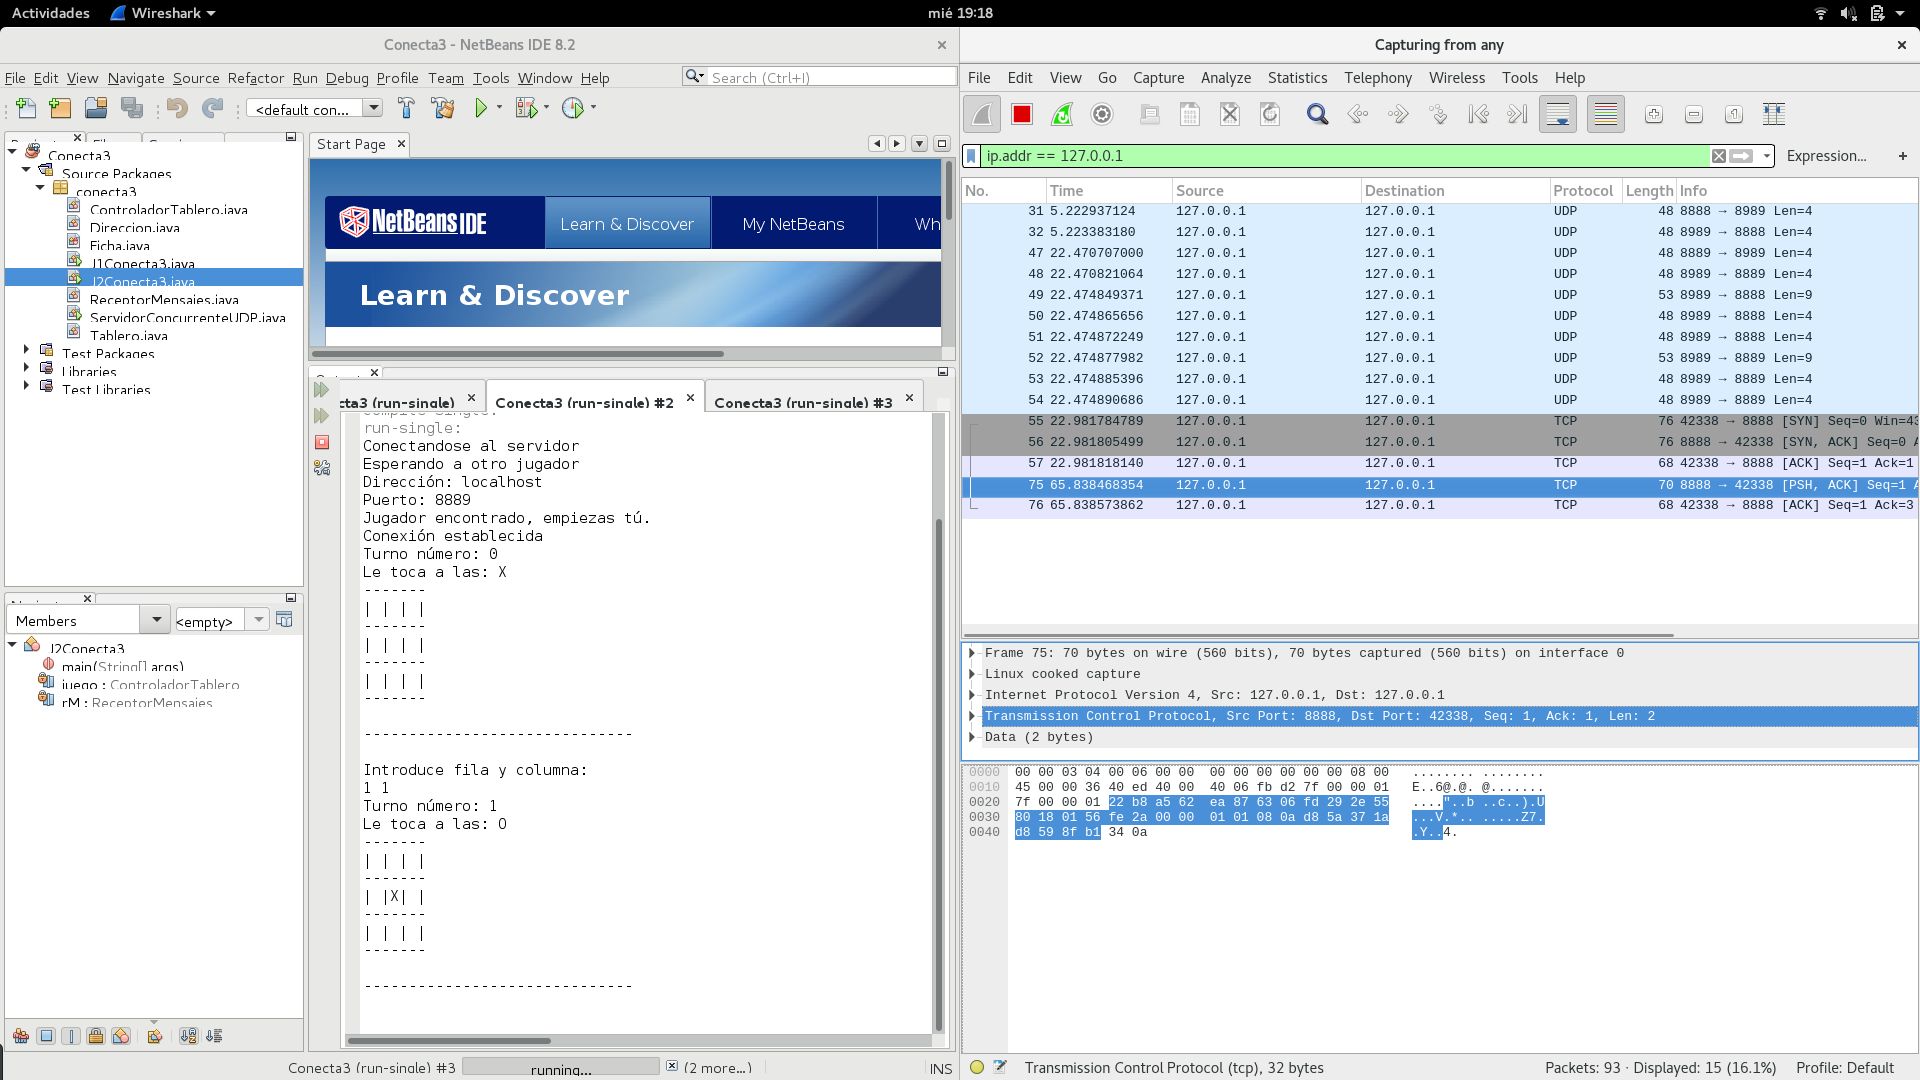
\includegraphics[width=0.9\textwidth]{3.png}
     \caption{Position sent}
     \end{figure}
\end{frame}

\section{Bibliography}
\begin{frame}
	\frametitle{Bibliography}
	References:
	\begin{itemize}
		\item Website: \href{https://www.gameranger.com/about/}{\beamergotobutton{Game Ranger}}
		\item Article: \href{https://gafferongames.com/post/udp_vs_tcp/}{\beamergotobutton{UDP vs TCP - Gaffer on Games}}
		\item Article: \href{https://1024monkeys.wordpress.com/2014/04/01/game-servers-udp-vs-tcp/}{\beamergotobutton{UDP vs TCP - 1024 Monkeys}}
		\item Article: \href{https://gafferongames.com/post/what_every_programmer_needs_to_know_about_game_networking/}{\beamergotobutton{Server types - Gaffer on Games}}
	\end{itemize}
\end{frame}

    
\end{document}
